\chapter{Pre-Verbal Affective Vector Projection}

The previous chapter established that, for a given target emotion $e$, the decomposed steering vector
\[
\Delta_e(\alpha_G,\alpha_R)=\alpha_G\mathbf{g}+\alpha_R\hat{\mathbf{r}}_e
\]
reliably shifts the affective framing of generated text towards $e$ while preserving semantic content.
In that framework, joy, sadness, anger, and the other Plutchik categories were treated as
\emph{primitive} units: each $\hat{\mathbf{r}}_e$ was taken to be an irreducible
emotion-specific direction without further decomposition.

This chapter re-examines that assumption.
The central question is whether named emotion categories such as \emph{joy} or \emph{fear}
are the minimal units of affective representation in the model's residual stream,
or whether each $\hat{\mathbf{r}}_e$ is itself a composite, structured along a small set of
more fundamental, pre-categorical affective dimensions.
The experiments reported here provide evidence for the latter: within each named emotion there
exist local sub-axes, these sub-axes are largely shared across emotion categories, and they can be
interpreted as dimensions that are more primitive than any named emotion label.
The central conclusion is that what Chapter~1 called $\hat{\mathbf{r}}_e$
can be re-read as a projection onto a shared pre-verbal affective space:
\[
\hat{\mathbf{r}}_e
\;=\;
\sum_{k=1}^{K}\beta_{e,k}\,\mathbf{m}_k
\;+\;
\boldsymbol{\varepsilon}_e,
\]
where $\mathbf{m}_k$ are label-free meta-axes shared across all emotions,
$\beta_{e,k}=\hat{\mathbf{r}}_e^\top\mathbf{m}_k$ are scalar projections that encode the
``affective fingerprint'' of emotion $e$, and $\boldsymbol{\varepsilon}_e$ is the residual
component that is orthogonal to all $\mathbf{m}_k$.

\section*{Experimental Roadmap}

This chapter is organised as follows.
\begin{enumerate}
  \item \textbf{Discriminability of $\hat{\mathbf{r}}_e$}: We first verify that the residual
    $\hat{\mathbf{r}}_e$ is a genuine emotion-specific signal rather than noise, motivating the
    search for its internal structure.
  \item \textbf{Internal variance structure}: We characterise the internal dimensionality of
    each named emotion by applying PCA to the distribution of per-source residual vectors
    within each emotion category.
  \item \textbf{Local sub-axis extraction and interpretation}: We extract the leading
    principal directions within each emotion and submit them to an LLM judge for semantic
    interpretation. We also confirm that these axes are affective rather than stylistic
    artefacts.
  \item \textbf{Cross-emotion sharing}: We show that the local PCA axes cluster by
    \emph{rank} rather than by emotion label, revealing a set of shared meta-axes
    $\mathbf{m}_k$ that span all named emotions.
  \item \textbf{Extraction and formalisation of meta-axes}: We formalise $\mathbf{m}_k$ as
    sign-aligned means over per-emotion PCA directions, and assess their stability.
  \item \textbf{Pre-verbal interpretation}: We interpret each $\mathbf{m}_k$ by presenting
    extreme examples from \emph{all} emotions simultaneously to an LLM judge, obtaining
    emotion-independent semantic labels for each meta-axis.
  \item \textbf{Re-decomposition of $\hat{\mathbf{r}}_e$}: We project each $\hat{\mathbf{r}}_e$
    onto the $\mathbf{m}_k$ basis, quantify the explained variance, and state the
    revised decomposition that extends the formula from Chapter~1.
  \item \textbf{Causal validation -- local axis steering}: We test whether adding
    $\pm\beta\,\mathbf{u}_{e,1}$ or $\pm\beta\,\mathbf{m}_1$ to the steering vector causally
    shifts outputs along the expected affective sub-dimension.
  \item \textbf{Label-free steering}: We compare three steering conditions---named emotion
    prototype only, $\mathbf{m}_k$-projection only, and their combination---to determine
    whether the $\mathbf{m}_k$ decomposition retains the practical utility of $\hat{\mathbf{r}}_e$.
\end{enumerate}

% ─────────────────────────────────────────────────────────────
\section{Geometric Overview of the Affective Residual Space}
\label{sec:ch2-geometry}

Before asking whether $\hat{\mathbf{r}}_e$ has internal sub-structure, we characterise the
geometry of the eight emotion-specific directions as a whole.
This provides a baseline picture of what kind of space $\hat{\mathbf{r}}_e$ lives in, and
motivates the specific questions that follow.

\subsection*{Raw directions are near-collinear}

At layer~13, the pairwise cosine similarities among the eight pooled CAA directions
$\mathbf{c}^{\mathrm{pool}}_e$ are extremely high.
The mean off-diagonal cosine is $0.986$, and even Plutchik opposite pairs
(e.g., joy--sadness, trust--disgust) have a mean cosine of $0.984$, nearly indistinguishable
from adjacent pairs ($0.988$).
This near-collinearity is the signature of the dominant shared component $\mathbf{g}$:
all eight directions point in almost the same direction because the largest component of
any emotional activation is simply the shift from neutral to emotional.

Despite this, PCA over the eight pooled directions reveals a low-dimensional but
non-trivial structure: the participation ratio is $3.61$, with
$\mathrm{EVR}_{\mathrm{PC1}}=0.437$ and $\mathrm{EVR}_{\mathrm{PC1\text{-}3}}=0.812$.
Even before any explicit decomposition, emotion directions do not fill eight independent
dimensions; they are organised within roughly three to four effective axes.

\subsection*{Residualisation exposes structured negative geometry}

After removing $\mathbf{g}$, the geometry changes qualitatively.
The residual directions $\mathbf{r}_e = \mathbf{c}_e - (\mathbf{c}_e^\top\mathbf{g})\mathbf{g}$
have a mean off-diagonal cosine of $-0.137$.
Plutchik opposite pairs become clearly negative on average ($-0.306$), while adjacent pairs
remain weakly positive ($+0.090$).
This sign reversal shows that the residual space encodes emotion-specific structure that
is consistent with Plutchik's theoretical organisation of emotions.

\begin{figure}[H]
  \centering
  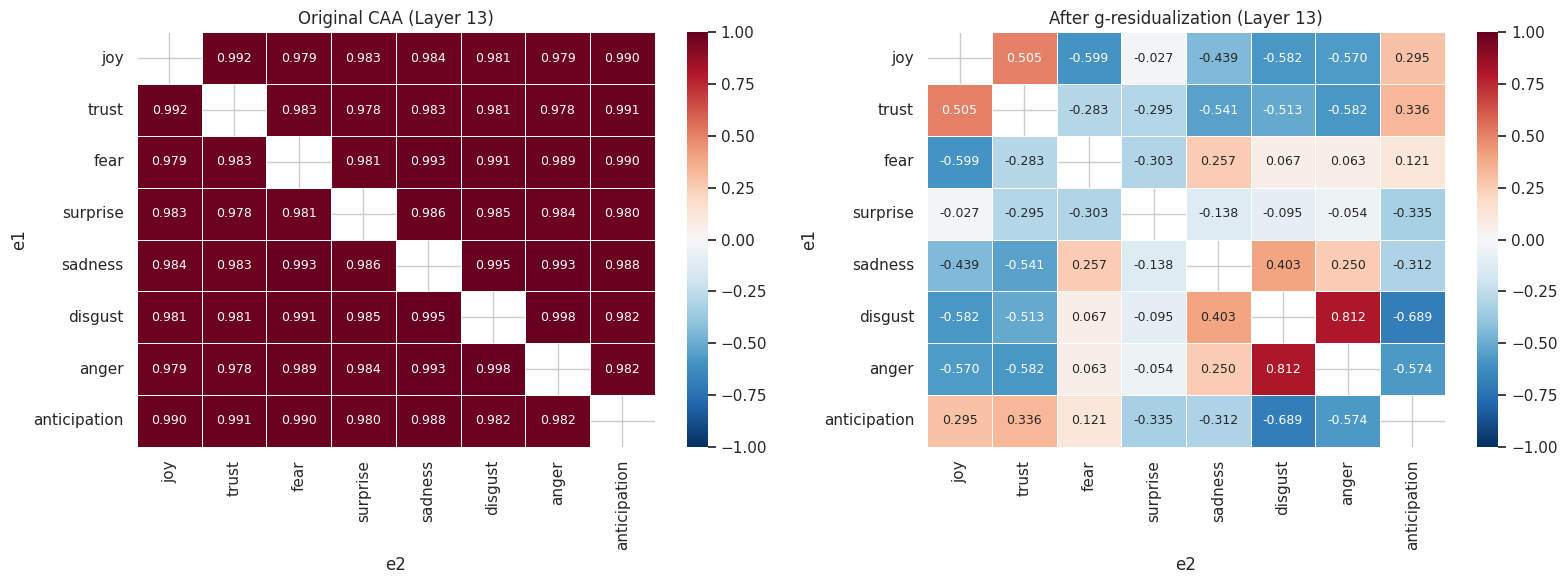
\includegraphics[width=0.80\linewidth]{figures/cosine_heatmap_before_after_L13.png}
  \caption{Pairwise cosine similarities among pooled CAA directions before (left) and
           after (right) removal of the shared emotionalisation component $\mathbf{g}$
           at layer~13. Before residualisation, all directions are near-collinear.
           After residualisation, Plutchik opposite pairs become negative and the
           emotion-specific structure is revealed.}
  \label{fig:cosine_before_after}
\end{figure}

\begin{figure}[H]
  \centering
  
\includegraphics[width=0.80\linewidth]{figures/plutchik_pairs_before_after.png}
  \caption{Mean cosine similarity of Plutchik opposite and adjacent emotion pairs
           across layers, before and after $\mathbf{g}$-residualisation.
           The crossover of opposite-pair cosines from positive to negative after
           residualisation is consistent across candidate layers.}
  \label{fig:plutchik_pairs}
\end{figure}

\subsection*{Residual directions are low-dimensional but internally heterogeneous}

Importantly, the residual space remains low-dimensional after this operation:
the participation ratio changes only from $3.61$ to $3.63$, and
$\mathrm{EVR}_{\mathrm{PC1}}=0.448$ for the eight $\mathbf{r}_e$ centroids.
This indicates that the emotion-specific information is not scattered across a
high-dimensional space but is organised within roughly four effective dimensions.

At the same time, per-source analysis reveals that the individual delta vectors
$\boldsymbol{\delta}_{n,e}$ within each named emotion are not tightly concentrated around their
centroid $\mathbf{r}_e$.
Local PCA within each emotion yields participation ratios of approximately $3.5$--$3.7$
(for the top-5 component analysis), and the first local PC accounts for only $11$--$12\%$
of intra-emotion variance.
In other words, while $\mathbf{r}_e$ is a good summary direction for emotion $e$, each
emotion behaves more like a \emph{cone} or a \emph{prototype region} with internal
sub-axes than like a single, thin direction.

\subsection*{The implication: r̂_e has internal structure worth investigating}

Together, these observations motivate the core question of this chapter.
The residual directions $\hat{\mathbf{r}}_e$ are meaningful (Plutchik geometry is
preserved), structured (low-dimensional), but internally heterogeneous (each emotion
spans a cone rather than a point).
The experiments that follow ask: what are the axes within each cone, are they shared
across emotions, and do they correspond to interpretable pre-verbal affective dimensions?

% ─────────────────────────────────────────────────────────────
\section{Discriminability of the Emotion-Specific Residual}
\label{sec:ch2-discriminability}

% Exp1: after removing g, r_e still decodes emotion labels at ~85% balanced accuracy.
% This section answers: is r_e meaningful beyond the emotionalisation component?

Before asking about the internal geometry of $\hat{\mathbf{r}}_e$, we first confirm that it
carries genuine emotion-specific information.
If $\hat{\mathbf{r}}_e$ were merely the small orthogonal complement of a dominant
emotionalisation direction and contained no structured signal, the internal analysis that
follows would be unmotivated.

\subsection*{Protocol}

For each source utterance $n$ and emotion $e$, we define the per-source affective shift
\[
\boldsymbol{\delta}_{n,e}
=\mathbf{h}^{\mathrm{emo}}_{n,e}-\mathbf{h}^{\mathrm{neu}}_{n},
\]
and remove the shared emotionalisation direction $\mathbf{g}$:
\[
\boldsymbol{\delta}^{g\perp}_{n,e}
=\boldsymbol{\delta}_{n,e}-(\boldsymbol{\delta}_{n,e}^\top\mathbf{g})\mathbf{g}.
\]
We then train a linear probe (PCA-64 $\to$ standardised logistic regression) to predict the
emotion label $e$ from $\boldsymbol{\delta}^{g\perp}_{n,e}$, using five-fold cross-validation
grouped by source identity to prevent leakage.
Chance level is $1/8=0.125$.

\subsection*{Results}

% Table: balanced accuracy by layer (from exp1)
\begin{table}[H]
\centering
\small
\begin{tabular}{lcc}
\toprule
\textbf{Layer} & \textbf{Balanced accuracy} & \textbf{Std} \\
\midrule
10 & 0.853 & 0.002 \\
13 \textbf{*} & \textbf{0.857} & 0.001 \\
16 & 0.755 & 0.002 \\
\bottomrule
\end{tabular}
\caption{Emotion-label balanced accuracy from a linear probe trained on
         $\boldsymbol{\delta}^{g\perp}_{n,e}$ (affective shift with shared emotionalisation
         removed). Asterisk marks the primary reporting layer selected in Chapter~1.
         Chance level is $0.125$.}
\label{tab:exp1_probe_accuracy}
\end{table}

At layer~13, balanced accuracy reaches $0.857$, nearly seven times the chance level.
This demonstrates that the g-residualised shifts contain strong, linearly decodable
emotion-category information independent of the shared emotionalisation component.
The signal peaks at layers~10--13 and decays monotonically at deeper layers, consistent with
a representation that is transformed from qualitative affective identity towards
next-token prediction at higher depths.

\subsection*{Interpretation}

The high discriminability of $\boldsymbol{\delta}^{g\perp}_{n,e}$ confirms that
$\hat{\mathbf{r}}_e$ is not noise.
It encodes the qualitative difference between \emph{joy}, \emph{sadness}, \emph{anger}, and
so on.
This motivates the next question: what is the internal geometric structure of these directions?

% ─────────────────────────────────────────────────────────────
\section{Internal Variance Structure of Named Emotions}
\label{sec:ch2-variance-structure}

% Exp2: per-emotion PCA, participation ratio analysis.
% joy/trust concentrated; fear/surprise diffuse.
% Named emotions differ in their internal dimensionality.

The previous section shows that $\hat{\mathbf{r}}_e$ is a genuine signal.
A single vector, however, summarises an entire distribution: for each emotion $e$, there are
$N \times I$ per-source residual vectors $\boldsymbol{\delta}^{g\perp}_{n,e,i}$, and $\hat{\mathbf{r}}_e$
is their normalised average.
This section asks whether the \emph{distribution} is concentrated around a single
direction or whether it spans multiple dimensions.

\subsection*{Protocol}

For each emotion $e$, we collect the per-source, per-intensity residuals
$\boldsymbol{\delta}^{g\perp}_{n,e,i}$ at layer~13, apply PCA, and compute the participation
ratio
\[
\mathrm{PR}_e
=\frac{\left(\sum_k \lambda_k\right)^2}{\sum_k \lambda_k^2},
\]
where $\lambda_k$ are the eigenvalues of the empirical covariance.
To establish a baseline, we shuffle the emotion labels to destroy emotion-specific structure
and report $\mathrm{PR}_{\mathrm{shuffle}}$.
A value $\mathrm{PR}_e < \mathrm{PR}_{\mathrm{shuffle}}$ indicates that the emotion's
internal distribution is \emph{more concentrated} than random, whereas
$\mathrm{PR}_e > \mathrm{PR}_{\mathrm{shuffle}}$ indicates a \emph{more diffuse}, multi-axis
structure.

\subsection*{Results}

% Table: participation ratio (from exp2)
\begin{table}[H]
\centering
\small
\begin{tabular}{lccc}
\toprule
\textbf{Emotion} & \textbf{PR} & \textbf{PR (shuffle)} & \textbf{PR excess} \\
\midrule
joy        &  6.72 & 13.62 & $-6.90$ \\
trust      & 10.54 & 13.65 & $-3.11$ \\
sadness    & 12.11 & 13.59 & $-1.48$ \\
disgust    & 12.74 & 13.61 & $-0.87$ \\
anticipation & 15.30 & 13.65 & $+1.65$ \\
anger      & 15.56 & 13.63 & $+1.93$ \\
fear       & 18.16 & 13.60 & $+4.57$ \\
surprise   & 18.94 & 13.63 & $+5.31$ \\
\bottomrule
\end{tabular}
\caption{Participation ratio of per-source affective shift distributions at layer~13.
         A negative excess indicates a concentrated, near-uniaxial structure;
         a positive excess indicates a diffuse, multi-axis structure.}
\label{tab:exp2_participation_ratio}
\end{table}

The results reveal a clear gradient: joy and trust have highly concentrated
internal distributions (PR well below shuffle), whereas fear and surprise are substantially
more diffuse (PR well above shuffle).
Named emotions are therefore not equivalent in their internal dimensionality: some are
almost prototype-like, while others occupy broader affective regions.

\subsection*{Interpretation}

Each named emotion category is not a single, thin direction but a cone or region with
its own internal geometry.
The variation across the $N \times I$ per-source residuals encodes sub-distinctions
within joy, within fear, and so on.
This internal structure is the subject of the next section.

% ─────────────────────────────────────────────────────────────
\section{Local Sub-Axes and Their Affective Interpretation}
\label{sec:ch2-local-axes}

% Exp3 + Exp4: PCA within each emotion's residuals → local sub-axes u_{e,k}.
% LLM judge interpretations. Style contamination check.

The participation ratio analysis shows that each named emotion has non-trivial internal
variation.
We now characterise this variation explicitly by extracting local principal axes.

\subsection*{Extraction pipeline}
\label{subsec:local-axis-pipeline}

Starting from the per-source affective shifts, we apply the following residualisation steps
before extracting emotion-internal principal components.

\begin{enumerate}
  \item Compute the base shift:
    $\boldsymbol{\delta}_{n,e,i} = \mathbf{h}^{\mathrm{emo}}_{n,e,i} - \mathbf{h}^{\mathrm{neu}}_{n}$.
  \item Remove the shared emotionalisation direction:
    $\boldsymbol{\delta}^{(1)}_{n,e,i} = \boldsymbol{\delta}_{n,e,i} - (\boldsymbol{\delta}_{n,e,i}^\top\mathbf{g})\mathbf{g}$.
  \item Remove the per-emotion intensity direction $\mathbf{u}_e$
    (the normalised mean of $\boldsymbol{\delta}^{(1)}_{n,e,\cdot}$ over intensities $i$):
    $\boldsymbol{\delta}^{(2)}_{n,e,i} = \boldsymbol{\delta}^{(1)}_{n,e,i} - (\boldsymbol{\delta}^{(1)}_{n,e,i}{}^\top\mathbf{u}_e)\mathbf{u}_e$.
  \item Remove source-wise mean (mean over emotions for the same source $n$):
    $\boldsymbol{\delta}^{(3)}_{n,e,i} = \boldsymbol{\delta}^{(2)}_{n,e,i} - \frac{1}{|E|}\sum_{e'}\boldsymbol{\delta}^{(2)}_{n,e',i}$.
\end{enumerate}

For each emotion $e$, we collect the matrix
$\{\boldsymbol{\delta}^{(3)}_{n,e,i}\}_{n,i}$ and apply PCA.
The $k$-th principal component is denoted $\mathbf{u}_{e,k}$; it is the direction of maximal
residual variance within emotion $e$ that is orthogonal to $\mathbf{g}$ and to $\mathbf{u}_e$.

\subsection*{Interpretation of local sub-axes}

We submit the top-5 and bottom-5 example texts for each $\mathbf{u}_{e,k}$ to an
LLM judge (GPT-4o) and ask it to label the axis semantically.
Table~\ref{tab:local_axis_pc1} summarises the leading axis for each emotion,
along with judge-assigned contamination and confidence scores.

% Table: PC1 interpretations (from exp3)
\begin{table}[H]
\centering
\small
\begin{tabular}{p{0.15\linewidth} p{0.47\linewidth} p{0.12\linewidth} p{0.12\linewidth}}
\toprule
\textbf{Emotion} & \textbf{PC1 axis name} & \textbf{Contam.} & \textbf{Conf.} \\
\midrule
joy          & Reflective/perspective-taking joy \emph{vs} immediate/external event joy       & medium & 4 \\
trust        & Trust as hopeful acceptance \emph{vs} self-assured confidence                   & medium & 5 \\
fear         & Immediate situational anxiety \emph{vs} chronic/existential worry               & low    & 5 \\
surprise     & Unexpected events \emph{vs} expected/anticipated events                         & low    & 5 \\
sadness      & Loss \& disappointment \emph{vs} everyday contentment                           & low    & 5 \\
disgust      & Visceral sensory repulsion \emph{vs} mild/abstract discomfort                   & medium & 4 \\
anger        & Irritation/frustration \emph{vs} disappointment/resigned upset                  & low    & 5 \\
anticipation & Hopeful curiosity \emph{vs} uneasy waiting                                      & low    & 5 \\
\bottomrule
\end{tabular}
\caption{LLM-judge interpretations of the leading local sub-axis $\mathbf{u}_{e,1}$ for each
         emotion at layer~13.
         Five of eight emotions achieve contamination = low and confidence = 5, indicating
         that the extracted axes capture genuine affective distinctions rather than stylistic
         variation.}
\label{tab:local_axis_pc1}
\end{table}

\subsection*{Style contamination check}
\label{subsec:style-contamination}

% Exp4: 34/40 axes classified as likely_affective; Methods A/B/C.

To confirm that the local axes are affective rather than artefacts of text style or topic,
we apply three independent checks to all 40 axes (8 emotions $\times$ 5 PCs).

\begin{itemize}
  \item \textbf{Method A (style-feature probe).} We regress the PC scores on a battery of
    surface features (sentence length, lexical diversity, POS ratios, etc.).
    Mean $R^2$ over 40 axes is $0.069$; only 5 axes exceed the threshold of $0.15$.
  \item \textbf{Method B (neutral-control alignment).} We extract PCA axes from the neutral
    paraphrase activations and measure cosine alignment with each local PC.
    Mean maximum cosine is $0.034$, uniformly low, indicating no systematic confound from
    paraphrase-level style variation.
  \item \textbf{Method C (meaning-preservation filter).} We restrict the analysis to
    rewrites that pass a semantic-similarity filter and recompute PCA axes.
    Mean cosine between full and filtered axes is $0.944$; only 1 of 40 axes
    ($\mathrm{surprise}\text{ PC5}$) drops below the robustness threshold of $0.70$.
\end{itemize}

Based on these three checks, 34 of 40 axes are classified as \textbf{likely affective},
6 as ambiguous, and none as likely stylistic.
The local PCA axes therefore reflect genuine sub-distinctions within the affective content of
each emotion category rather than co-varying surface features.

% ─────────────────────────────────────────────────────────────
\section{Cross-Emotion Sharing: From Local Axes to Meta-Axes}
\label{sec:ch2-meta-axes}

% Exp6: clustering shows PC-rank, not emotion-label, determines similarity.
% Exp7: formalise m_k.

So far, the local sub-axes $\mathbf{u}_{e,k}$ have been characterised separately for each
emotion.
We now ask whether these axes are emotion-specific or whether they encode dimensions that
recur across emotions.
This turns out to be a crucial question: if the sub-axes are shared, then the internal
variation of each named emotion is organised along the same underlying dimensions,
and $\hat{\mathbf{r}}_e$ can be re-read as a specific pattern of activations along those
shared dimensions.

\subsection*{Clustering reveals PC-rank, not emotion label, as the organising principle}

% Exp6 main result
We compute the absolute cosine similarity between all 40 local PC vectors (8 emotions $\times$
5 PCs) and apply Ward hierarchical clustering.
The resulting dendrogram reveals a striking pattern: the dominant clusters group axes by
their \emph{rank} ($k=1,2,3$) rather than by emotion label.
Specifically:
\begin{itemize}
  \item The $k=1$ axes of all eight emotions form a single, tight cluster
    ($|\cos|\approx 0.74$--$0.95$ across all pairs).
  \item The $k=2$ axes of all eight emotions form a second cluster.
  \item The $k=3$ axes similarly form a third cluster.
  \item Emotion-specific structure first appears at $k=4$ and $k=5$.
\end{itemize}

This organisation is confirmed by cross-emotion cosine similarities at the PC1 level
(Table~\ref{tab:cross_emotion_cosine_pc1}) and by meta-PCA over the 40 vectors,
where the top-3 meta-components capture 51\% of the total variance across
all emotion-PC combinations and separate by rank.

\begin{table}[H]
\centering
\small
\begin{tabular}{lcc}
\toprule
\textbf{Emotion pair (PC1)} & $|\cos(\mathbf{u}_{e_1,1},\mathbf{u}_{e_2,1})|$ \\
\midrule
disgust -- anger    & 0.950 \\
sadness -- disgust  & 0.922 \\
trust   -- disgust  & 0.886 \\
joy     -- anger    & 0.874 \\
fear    -- disgust  & 0.839 \\
anticipation -- sadness & 0.805 \\
surprise -- sadness & 0.743 \\
\bottomrule
\end{tabular}
\caption{Cross-emotion absolute cosine similarity for the leading local sub-axis
         $\mathbf{u}_{e,1}$. All pairs are well above chance, indicating a universal
         primary axis shared across all eight named emotions.}
\label{tab:cross_emotion_cosine_pc1}
\end{table}

\subsection*{Formalisation of meta-axes $\mathbf{m}_k$}
\label{subsec:meta-axis-def}

% Exp7: sign-aligned mean, method agreement
Given that $k$-th rank local axes cluster tightly across emotions, we define a shared
\textbf{meta-axis} $\mathbf{m}_k$ as the normalised sign-aligned mean of the $k$-th local
PC vectors:
\[
\mathbf{m}_k
=\frac{\sum_{e\in E}\sigma_{e,k}\,\mathbf{u}_{e,k}}
      {\left\lVert\sum_{e\in E}\sigma_{e,k}\,\mathbf{u}_{e,k}\right\rVert_2},
\]
where $\sigma_{e,k}\in\{+1,-1\}$ is chosen by sign-aligning $\mathbf{u}_{e,k}$ with the
first emotion's axis so that all vectors point in a consistent direction before averaging.

As a robustness check, we also extract $\mathbf{m}_k$ via group PCA (applying PCA to the
sign-aligned set of $k$-th rank vectors) and measure the cosine between the two estimates.

\begin{table}[H]
\centering
\small
\begin{tabular}{lcc}
\toprule
\textbf{Meta-axis} & $|\cos(\mathbf{m}_k^{\mathrm{mean}},\mathbf{m}_k^{\mathrm{pca}})|$
  & \textbf{Mean $|\cos|$ to $\mathbf{u}_{e,k}$} \\
\midrule
$\mathbf{m}_1$ & 0.990 & 0.892 \\
$\mathbf{m}_2$ & 0.829 & 0.800 \\
$\mathbf{m}_3$ & 0.989 & 0.672 \\
$\mathbf{m}_4$ & 0.266 & 0.437 \\
$\mathbf{m}_5$ & 0.104 & 0.427 \\
\bottomrule
\end{tabular}
\caption{Stability of meta-axes $\mathbf{m}_k$. The first column reports agreement between
         the two extraction methods (sign-aligned mean vs.\ group PCA); the second reports
         mean absolute cosine between $\mathbf{m}_k$ and the individual local axes
         $\mathbf{u}_{e,k}$.
         Meta-axes $\mathbf{m}_1$--$\mathbf{m}_3$ are stable and representative;
         $\mathbf{m}_4$ and $\mathbf{m}_5$ are not.}
\label{tab:meta_axis_stability}
\end{table}

Meta-axes $\mathbf{m}_1$, $\mathbf{m}_2$, and $\mathbf{m}_3$ are stable under
method variation (method agreement $\geq 0.83$) and well-aligned with the individual local
axes (mean $|\cos| \geq 0.67$).
Meta-axes $\mathbf{m}_4$ and $\mathbf{m}_5$ show poor method agreement ($0.27$ and $0.10$)
and are excluded from further interpretation.

Two additional properties of the stable meta-axes are noteworthy.
First, all $\mathbf{m}_k$ are nearly orthogonal to the shared emotionalisation direction
$\mathbf{g}$ ($|\cos(\mathbf{m}_k,\mathbf{g})| < 0.02$ for all $k$), confirming that they
capture \emph{affective texture} rather than overall emotionalisation strength.
Second, all $\mathbf{m}_k$ are nearly orthogonal to each named emotion's steering residual
$\hat{\mathbf{r}}_e$ ($|\cos(\mathbf{m}_k,\hat{\mathbf{r}}_e)| < 0.09$ for all combinations),
which means that the meta-axes are not recoverable from the averaged prototype alone -- they
encode within-emotion variance that the averaging operation obscures.

% ─────────────────────────────────────────────────────────────
\section{Pre-Verbal Interpretation of Meta-Axes}
\label{sec:ch2-preverbal-interp}

% Exp8 v2: contrastive LLM judge, all emotions simultaneously.
% m1=arousal/reactivity, m2=temporal, m3=social/internal, m4=meaning, m5=relief/tension.

We now ask what affective dimension each meta-axis $\mathbf{m}_k$ represents.
Because the meta-axes are derived from activations aggregated \emph{across} all named
emotions, their semantic content should be describable without reference to any specific
emotion label.
We therefore present extreme activation examples drawn from \emph{all eight emotions}
simultaneously to an LLM judge (GPT-4.1), with the explicit instruction that the labels
assigned to the five axes must be mutually distinct and must describe what differentiates
the high pole from the low pole \emph{across emotion categories}.
This contrastive evaluation is designed to surface dimensions that are more primitive than
emotion labels, rather than the within-emotion nuances captured in Section~\ref{sec:ch2-local-axes}.

\subsection*{Results}

\begin{table}[H]
\centering
\small
\begin{tabular}{p{0.05\linewidth} p{0.30\linewidth} p{0.40\linewidth} p{0.10\linewidth} p{0.06\linewidth}}
\toprule
& \textbf{Axis name} & \textbf{Pre-verbal interpretation} & \textbf{Contam.} & \textbf{Conf.} \\
\midrule
$\mathbf{m}_1$ & Agitated/reactive \emph{vs} mellow/accepting
  & Arousal / affective reactivity: how strongly and immediately a state is felt
  & medium & 5 \\
$\mathbf{m}_2$ & Nostalgic/ruminative \emph{vs} pragmatic/forward-looking
  & Temporal orientation: backward-looking rumination vs.\ present-focused pragmatic coping
  & medium & 4 \\
$\mathbf{m}_3$ & Interpersonally engaged / closure-seeking \emph{vs} self-contained / processing
  & Social vs.\ internal orientation: whether affect is directed outward or processed internally
  & medium & 4 \\
$\mathbf{m}_4$ & Mundane/obligatory \emph{vs} meaningful/fulfilling
  & Existential weight: trivial routine vs.\ personally significant experience
  & medium & 4 \\
$\mathbf{m}_5$ & Relief/release \emph{vs} tension/constraint
  & Somatic pressure: physical or situational release vs.\ constriction
  & medium & 5 \\
\bottomrule
\end{tabular}
\caption{LLM-judge interpretation of the five meta-axes at layer~13.
         Labels are derived from contrastive evaluation across all eight named emotions
         simultaneously, yielding emotion-independent descriptions.
         Contamination is medium for all axes, reflecting the inherent ambiguity of
         cross-emotion generalisation; confidence is 4--5.}
\label{tab:meta_axis_interpretations}
\end{table}

The five dimensions correspond to established constructs in emotion psychology:
$\mathbf{m}_1$ maps onto the arousal dimension of Russell's circumplex model;
$\mathbf{m}_2$ maps onto temporal orientation in rumination theory
(Nolen-Hoeksema);
$\mathbf{m}_3$ corresponds to the social sharing of emotions (Rim\'e);
$\mathbf{m}_4$ relates to the relevance and significance appraisal in appraisal theory;
and $\mathbf{m}_5$ resembles Damasio's somatic marker gradient.
None of these dimensions is emotion-specific: each spans all eight named categories and
can be varied independently of the emotion label.

% ─────────────────────────────────────────────────────────────
\section{Re-Interpreting $\hat{\mathbf{r}}_e$ as a Pre-Verbal Projection}
\label{sec:ch2-reinterpretation}

% THE KEY SECTION.
% r_e = Σ_k β_{e,k} m_k + ε_e
% β_{e,k} = r_e · m_k, explains ~22% of r_e on average.
% Named emotions are patterns in pre-verbal space.

The experiments so far establish that (i) each named emotion has internal sub-axes,
(ii) these sub-axes are shared across emotion categories, and (iii) the shared meta-axes
have pre-verbal, emotion-independent interpretations.
This section draws these threads together into a revised decomposition of $\hat{\mathbf{r}}_e$.

\subsection*{Decomposition}

Each meta-axis $\mathbf{m}_k$ defines a direction in residual space.
For a given emotion $e$, we define the \textbf{projection coefficient}
\[
\beta_{e,k} = \hat{\mathbf{r}}_e^\top\mathbf{m}_k
\]
and write the decomposition
\[
\hat{\mathbf{r}}_e
= \underbrace{\sum_{k=1}^{K}\beta_{e,k}\,\mathbf{m}_k}_{\text{pre-verbal projection}}
+ \underbrace{\boldsymbol{\varepsilon}_e}_{\text{emotion-specific residual}},
\]
where $\boldsymbol{\varepsilon}_e \perp \mathbf{m}_k$ for all $k$, and
$K=5$ (all extracted meta-axes; recall that $\mathbf{m}_1$--$\mathbf{m}_3$ are stable
while $\mathbf{m}_4$, $\mathbf{m}_5$ have lower method agreement).
The explained variance ratio is
$\mathrm{EVR}(e) = \sum_{k=1}^{K}\beta_{e,k}^2$
(since $\hat{\mathbf{r}}_e$ is a unit vector).

\subsection*{Results}

\begin{table}[H]
\centering
\small
\begin{tabular}{lrrrrrr}
\toprule
\textbf{Emotion} & $\beta_{e,1}$ & $\beta_{e,2}$ & $\beta_{e,3}$ & $\beta_{e,4}$ & $\beta_{e,5}$ & \textbf{EVR} \\
\midrule
joy          & $+0.160$ & $-0.261$ & $-0.073$ & $+0.156$ & $+0.269$ & 0.238 \\
trust        & $-0.062$ & $-0.249$ & $+0.152$ & $-0.211$ & $+0.235$ & 0.185 \\
fear         & $-0.442$ & $+0.060$ & $+0.162$ & $-0.073$ & $-0.102$ & 0.231 \\
surprise     & $+0.224$ & $+0.553$ & $-0.256$ & $-0.083$ & $-0.043$ & 0.399 \\
sadness      & $+0.070$ & $+0.174$ & $-0.089$ & $+0.429$ & $-0.227$ & 0.263 \\
disgust      & $-0.041$ & $+0.041$ & $-0.151$ & $+0.066$ & $-0.295$ & 0.125 \\
anger        & $-0.034$ & $-0.008$ & $+0.035$ & $-0.060$ & $-0.242$ & 0.058 \\
anticipation & $+0.050$ & $-0.319$ & $+0.236$ & $-0.083$ & $+0.247$ & 0.227 \\
\midrule
\textbf{Mean} &        &          &          &          &          & \textbf{0.216} \\
\bottomrule
\end{tabular}
\caption{Projection coefficients $\beta_{e,k}=\hat{\mathbf{r}}_e^\top\mathbf{m}_k$ and
         explained variance ratio (EVR) across all five meta-axes.
         The $\beta_{e,k}$ pattern constitutes the ``affective fingerprint'' of each
         named emotion in the pre-verbal meta-axis space.
         All five meta-axes together explain approximately 22\% of the variance
         in $\hat{\mathbf{r}}_e$; the remaining 78\% is the emotion-specific residual
         $\boldsymbol{\varepsilon}_e$.}
\label{tab:beta_coefficients}
\end{table}

Several patterns in the $\beta_{e,k}$ coefficients are interpretable.
Fear has the most negative $\beta_{e,1}$ ($-0.442$), placing it firmly toward the
calm/detached pole of the arousal meta-axis --- a finding consistent with fear as
a state of vigilant suppression rather than overt agitation.
Surprise has the largest positive $\beta_{e,2}$ ($+0.553$), anchoring it at the
ruminative end of the temporal orientation axis, reflecting the retrospective quality
of processing an unexpected event.
Sadness has the largest $\beta_{e,4}$ ($+0.429$), corresponding to the meaningful/fulfilling
end of the existential weight axis, consistent with sadness framing loss as personally
significant.
Anticipation has the most negative $\beta_{e,2}$ ($-0.319$), placing it at the
pragmatic/forward-looking pole and contrasting with surprise's retrospective orientation
despite both involving uncertainty.
Joy is characterised primarily by $\beta_{e,5}=+0.269$ (release/relief) and
$\beta_{e,2}=-0.261$ (forward-looking), reflecting a state of positive resolution rather
than agitation.
Trust splits across $\beta_{e,2}=-0.249$ (forward-looking) and
$\beta_{e,4}=-0.211$ (routine/obligatory), suggesting that trust is encoded as pragmatic,
low-stakes acceptance rather than profound personal significance.

\subsection*{Connecting to Chapter 1}

We can now state the revised decomposition at the level of the steering vector.
Chapter~1 used the unit-normalised residual $\hat{\mathbf{r}}_e$ as the primitive
emotion-specific direction:
\[
\Delta_e(\alpha_G,\alpha_R)=\alpha_G\mathbf{g}+\alpha_R\hat{\mathbf{r}}_e.
\tag{Chapter 1}
\]
Chapter~2 decomposes $\hat{\mathbf{r}}_e$ into a pre-verbal projection and an orthogonal
emotion-specific residual:
\[
\hat{\mathbf{r}}_e = \sum_{k=1}^{K}\beta_{e,k}\,\mathbf{m}_k + \boldsymbol{\varepsilon}_e,
\qquad \beta_{e,k}=\hat{\mathbf{r}}_e^\top\mathbf{m}_k,
\qquad \boldsymbol{\varepsilon}_e\perp\mathbf{m}_k.
\tag{Chapter 2}
\]
Substituting into the steering formula:
\[
\Delta_e
= \alpha_G\mathbf{g}
  + \underbrace{\alpha_R\!\sum_{k=1}^{K}\beta_{e,k}\,\mathbf{m}_k}_{\text{pre-verbal component}}
  + \underbrace{\alpha_R\boldsymbol{\varepsilon}_e}_{\text{emotion-specific residual}}.
\tag{Combined}
\]
The practical question is whether the $\alpha_R\boldsymbol{\varepsilon}_e$ term contributes
useful signal or noise.
This is answered directly in Section~\ref{sec:ch2-label-free-steering}: Condition~A steers
with the full $\alpha_R\hat{\mathbf{r}}_e$ (which includes $\boldsymbol{\varepsilon}_e$), while
Condition~B steers with only $\alpha_R\sum_k\beta_{e,k}\mathbf{m}_k$ (which excludes it).
Their comparison is therefore a direct empirical test of $\boldsymbol{\varepsilon}_e$'s
functional role.

In sum, what Chapter~1 called $\hat{\mathbf{r}}_e$ is not a primitive atom.
Named emotions are reinterpreted as \emph{specific patterns of activation} along
label-free pre-verbal dimensions $\mathbf{m}_k$, encoded by the fingerprint
$(\beta_{e,1},\dots,\beta_{e,K})$ in Table~\ref{tab:beta_coefficients}.

% ─────────────────────────────────────────────────────────────
\section{Causal Validation: Local Axis Steering}
\label{sec:ch2-local-steering}

% Exp5 + Exp9: steering along u_{e,1} and m_1.
% local_axis_match results, pole asymmetry.

The internal axes identified by PCA are geometric features of the activation distribution.
To establish that they are also \emph{causally} relevant to generation, we directly steer
along them and measure whether the outputs shift in the expected affective direction.

\subsection*{Steering formula}

We extend the Chapter~1 intervention to include a local axis component:
\[
\Delta_e(\alpha_G,\alpha_R,\beta)
= \alpha_G\mathbf{g}+\alpha_R\hat{\mathbf{r}}_e \pm \beta\,\mathbf{u}_{e,1},
\]
where $+\beta$ steers toward the high pole of the axis and $-\beta$ toward the low pole.
In a parallel condition, we substitute the shared meta-axis $\mathbf{m}_1$ for the
emotion-specific $\mathbf{u}_{e,1}$.

\subsection*{Results}

% Table from exp5: per-emotion local_axis_match
\begin{table}[H]
\centering
\small
\begin{tabular}{lccccc}
\toprule
\textbf{Emotion} & \textbf{$n$} & \textbf{local\_axis\_match}
  & \textbf{target\_match} & \textbf{fluency} & \textbf{style\_contam.} \\
\midrule
anger        & 48 & \textbf{0.445} & 0.242 & 0.906 & 0.667 \\
anticipation & 48 & 0.305 & 0.411 & 0.844 & 0.631 \\
fear         & 48 & 0.307 & 0.388 & 0.842 & 0.626 \\
joy          & 48 & 0.279 & 0.405 & 0.790 & 0.591 \\
sadness      & 48 & 0.258 & 0.340 & 0.884 & 0.630 \\
surprise     & 48 & 0.261 & 0.280 & 0.762 & 0.566 \\
trust        & 48 & 0.184 & 0.259 & 0.814 & 0.610 \\
disgust      & 48 & 0.163 & 0.213 & 0.883 & 0.654 \\
\bottomrule
\end{tabular}
\caption{LLM-judge evaluation of local-axis steering ($\pm\beta\,\mathbf{u}_{e,1}$)
         at layer~13 (Exp~5). Eight emotions, 24 seed texts, 2 poles.
         \emph{local\_axis\_match} is the judge's score for the intended sub-axis shift;
         \emph{target\_match} is the overall emotion match.
         Fluency remains high throughout.}
\label{tab:exp5_steering_results}
\end{table}

Steering along the local axis produces detectable affective shifts for most emotions,
with anger achieving the strongest \emph{local\_axis\_match} (0.445) despite using a
conservative $\beta=0.35$.
An important asymmetry emerges at the pole level: for anger, the low pole (calm/resigned)
produces a local axis match of 0.602, whereas the high pole (agitated/reactive) yields only
0.289.
This suggests that the base model's generation tendencies are asymmetrically distributed
along the meta-axis, a point revisited in Section~\ref{sec:ch2-label-free-steering}.

When the emotion-specific $\mathbf{u}_{e,1}$ is replaced by the shared $\mathbf{m}_1$,
overall performance is comparable
(target match: $0.923$ vs $0.926$, local axis match: $0.519$ vs $0.525$),
demonstrating that the shared meta-axis captures the essential causal component of the
local sub-axis.

% ─────────────────────────────────────────────────────────────
\section{Label-Free Affective Steering}
\label{sec:ch2-label-free-steering}

% Exp10: conditions A (r_e only), B (β_k m_k), C (r_e + m_k).
% B ≥ A in quality; C < B (ε_e is noise).
% Practical implication: steering with Σ β_{e,k} m_k is sufficient.

The Combined formula in Section~\ref{sec:ch2-reinterpretation} isolates a specific
empirical question: is $\boldsymbol{\varepsilon}_e$ -- the 78\% of $\hat{\mathbf{r}}_e$
that cannot be expressed via $\mathbf{m}_k$ -- functionally useful for steering,
or is it inert noise?
This experiment is designed to answer that question directly by constructing three
steering conditions that differ only in whether and how $\boldsymbol{\varepsilon}_e$ is included.

\subsection*{Three steering conditions}

We compare three steering conditions using the same coefficient magnitudes:
\begin{description}
  \item[Condition A (named prototype)] $\Delta = \alpha_G\mathbf{g}+\alpha_R\hat{\mathbf{r}}_e$.
    Since $\hat{\mathbf{r}}_e = \sum_k\beta_{e,k}\mathbf{m}_k + \boldsymbol{\varepsilon}_e$,
    this steers with \emph{both} the pre-verbal projection and $\boldsymbol{\varepsilon}_e$.
    Equivalent to the Chapter~1 intervention.
  \item[Condition B (label-free projection)]
    $\Delta = \alpha_G\mathbf{g}+\sum_k\tilde{\beta}_{e,k}\,\mathbf{m}_k$,
    where $\tilde{\beta}_{e,k}=\alpha_R\beta_{e,k}=\alpha_R(\hat{\mathbf{r}}_e^\top\mathbf{m}_k)$.
    This steers with only the $\mathbf{m}_k$-projection of $\hat{\mathbf{r}}_e$,
    \emph{explicitly excluding} $\boldsymbol{\varepsilon}_e$.
    The difference A$-$B therefore isolates the causal contribution of $\boldsymbol{\varepsilon}_e$.
  \item[Condition C (hybrid)] $\Delta = \alpha_G\mathbf{g}+\alpha_R\hat{\mathbf{r}}_e+\sum_k\tilde{\beta}_{e,k}\,\mathbf{m}_k$,
    which adds the meta-axis projection on top of the full named prototype.
    Since $\hat{\mathbf{r}}_e$ already contains the $\mathbf{m}_k$ component,
    this condition double-weights the pre-verbal projection relative to $\boldsymbol{\varepsilon}_e$.
\end{description}

\subsection*{Results}

\begin{table}[H]
\centering
\small
\begin{tabular}{lcccccc}
\toprule
\textbf{Metric} & \textbf{A} & \textbf{B} & \textbf{C} & \textbf{B$-$A} & \textbf{C$-$A} \\
\midrule
target emotion match    & 0.936 & \textbf{0.938} & 0.935 & $+0.002$ & $-0.001$ \\
meaning preservation    & 0.881 & \textbf{0.902} & 0.879 & $+0.021$ & $-0.002$ \\
fluency                 & 0.820 & \textbf{0.891} & 0.793 & $+0.071$ & $-0.027$ \\
style contamination     & 0.699 & \textbf{0.735} & 0.690 & $+0.036$ & $-0.009$ \\
subtle affective state  & 0.712 & \textbf{0.723} & 0.686 & $+0.011$ & $-0.026$ \\
label-free nuance       & 0.678 & \textbf{0.697} & 0.650 & $+0.019$ & $-0.028$ \\
\bottomrule
\end{tabular}
\caption{Comparison of three steering conditions on 24 seed texts at layer~13 (Exp~10).
         Condition B (label-free $\mathbf{m}_k$ projection) matches or exceeds Condition A
         (named emotion prototype) on all metrics, with a particularly notable improvement in
         fluency ($+0.071$).
         Condition C (hybrid) falls below both A and B, indicating that adding
         $\boldsymbol{\varepsilon}_e$ to the meta-axis projection reduces quality rather than
         enhancing it.}
\label{tab:exp10_abc_comparison}
\end{table}

Condition B achieves the same target-emotion match as Condition A (0.938 vs 0.936) while
producing noticeably more natural outputs (fluency: 0.891 vs 0.820).
Condition C, which adds the full $\hat{\mathbf{r}}_e$ on top of the meta-axis projection,
is worse than both A and B on every metric.
This pattern implies that the $\boldsymbol{\varepsilon}_e$ component -- the part of $\hat{\mathbf{r}}_e$
orthogonal to all $\mathbf{m}_k$ -- does not provide additional affective nuance but
introduces noise that degrades output fluency and naturalness.

The emotion-wise breakdown reveals one important exception: surprise degrades under Condition B
(fluency $-0.180$, style contamination $-0.213$), consistent with the earlier observation
that surprise has the highest participation ratio (PR excess $+5.31$) and the lowest
alignment between its local axes and the shared meta-axes.
This suggests that surprise has genuine emotion-specific structure in its $\boldsymbol{\varepsilon}_e$
component that is not captured by $\mathbf{m}_k$.

\subsection*{Interpretation}

The results support the following refined view of emotion representation:
named emotion labels function as convenient short-hands for specific activation
\emph{patterns} in the pre-verbal meta-axis space.
The $\beta_{e,k}$ values in Table~\ref{tab:beta_coefficients} are the core content of the
emotion label; the named prototype $\hat{\mathbf{r}}_e$ is largely recoverable from these
projections, and the residual $\boldsymbol{\varepsilon}_e$ is mostly non-functional for
generation.
Steering with $\sum_k\beta_{e,k}\mathbf{m}_k$ is therefore not only theoretically cleaner
but also empirically superior in terms of output quality.

% ─────────────────────────────────────────────────────────────
\section{Limitations and Transition}
\label{sec:ch2-limitations}

The experiments in this chapter establish that the emotion-specific residual $\hat{\mathbf{r}}_e$
from Chapter~1 has a structured internal geometry.
Its principal variance is organised along shared meta-axes $\mathbf{m}_k$ that have
pre-verbal, label-free interpretations.
The decomposition $\hat{\mathbf{r}}_e = \sum_k\beta_{e,k}\mathbf{m}_k + \boldsymbol{\varepsilon}_e$
extends the Chapter~1 formula into a three-level hierarchy:
shared emotionalisation ($\mathbf{g}$), pre-verbal affective dimensions ($\mathbf{m}_k$),
and a small emotion-specific residual ($\boldsymbol{\varepsilon}_e$).

Several limitations qualify these conclusions.

First, the meta-axis projection explains only approximately 22\% of the variance in
$\hat{\mathbf{r}}_e$; the remaining 78\% is $\boldsymbol{\varepsilon}_e$.
Although the label-free steering experiment (Section~\ref{sec:ch2-label-free-steering})
provides empirical evidence that $\boldsymbol{\varepsilon}_e$ contributes noise rather than
signal for most emotions, this does not mean $\boldsymbol{\varepsilon}_e$ is semantically
empty.
It may encode emotion-specific information that is relevant under different generation
conditions, at different coefficient scales, or for certain emotions (notably surprise, which
is the one case where Condition~A outperforms Condition~B).
The current evidence establishes that $\boldsymbol{\varepsilon}_e$ is functionally inert
\emph{under the tested conditions}, not that it is categorically meaningless.

Second, the LLM judge labels for $\mathbf{m}_k$ carry a contamination rating of medium,
reflecting the inherent difficulty of cross-emotion generalisation; the interpretation is
plausible but not independently verified by human raters or psychometric instruments.

Third, the evidence is based on a single model (Llama-3.1-8B-Instruct) and a single layer
(13); the generalisability of the meta-axis structure to other models or depths requires
further investigation.

Fourth, meta-axes $\mathbf{m}_4$ and $\mathbf{m}_5$ are unstable (method agreement $< 0.3$)
and are included only in the EVR computation; they are not used as interpretable axes.

These limitations motivate the next chapter.
The label-free $\mathbf{m}_k$ axes provide a principled basis for an affective interface
that is not tied to fixed emotion labels.
The next chapter asks how such a pre-verbal representation can be operationalised in a
practical user interface, and whether the decoupling of emotionalisation ($\mathbf{g}$),
affective texture ($\mathbf{m}_k$), and emotion-specific identity ($\boldsymbol{\varepsilon}_e$)
translates into meaningful and controllable user-facing controls.
